\section{Experiment 2}\label{sec:experiment_2}
This section will describe the second experiment of the project. The second experiment covers how many dimensions are necessary to still have a good accuracy of arround 95\%\todo{lower this to something more resonable}. The experiment will only be done on 15.000 samples, instead of the entire data set of 60.000 samples, due to issues regarding memory usage. The experimant will focus on when different dimensionality reduction methods, show a noticable drop in accuracy due to too few dimensions. 


\subsection{Rules and evaluation of the experiment}\label{subsec:experiment_2_rules}
This section will cover the rules of the second experiment, and also how the results of the experiment will be evaluated.

The second experiment is done on a subset of the entire data set. With 15.000 samples in the training set, and the usual 10.000 samples in the test set. Instead of the standard 60.000 samples in the training set and 10.000 in the test set.\todo{Remember to discuss why only a limited amount of the data set and give detailed reasons and difficulties}

The values from the \gls{mnist} dataset will be normalized using standard scalar, for each of the dimensionality reduction methods. This is to ensure that the values are on the same scale, so that the results are not skewed by different scales.\todo{Discussion?}

There will be done hyperparamater tuning, using gridsearch, on each of the dimensionality reduction methods. This is to ensure that good hyperparamaters are found for each number of components, so that the results are not sqewed by hyperparamaters that are not optimal for the number of components. If it was chosen to use fixed value for the hyperparamaters, the results could be skewed for some certain number of components.\todo{Discussion?}

The dimensionality reduction methods that will be used are \gls{pca}, \gls{lda}, \gls{isomap} and \gls{kpca}. The number of components will be varied from 2 to 50.\todo{Remember to discuss why this range} \gls{lda} is an exception, as the maximum number of components is the number of classes, which is 10 for the \gls{mnist} dataset.\todo{Ensure it is 10 and not 9} Meaning that the range of components for \gls{lda} will be from 2-10.

The values that will be used to evaluate this experiment, are the \texttt{mean\_fit\_time} to evaluate the time it takes to fit the model, the \texttt{mean\_test\_score} based on \texttt{param\_pca\_\_n\_components} to evaluate the accuracy of the modele with the number of components used.

With the results from running the experiment, a plot will be made to show the accuracy of the models with the number of components used. The plot is used to visually represent when the accuracy starts to drop. 

Depending on the usecase of the data, the loss of accuracy compared to the time saved, can vary. For each of the experiments, the data will be analyzed to see how many components can be removed, before the accuracy drops below a certain threshold, for the sake of the experiment different thresholds will be used that are based on the higest value of accuracy for each of the methods. The thresholds will be, a 1\% loss in accuracy, a 5\% loss in accuracy and a 10\% loss in accuracy. The results of the experiment will be compared to the thresholds, and the results will be evaluated based on the rules of the experiment.


\subsection{Results}\label{subsec:experiment_2_results}
This section will cover the results gathered from running the second experiment. Each of the dimensionality reduction methods will be presented using scatter plots. The scatter plots will show the number of components used along the x-axis, and the accuracy of the model along the y-axis. The results will then be compared, and evaluated based on the rules of the experiment. The main focus of the evaluation will be on when the accuracy starts to noticablly drop, and how many components are needed to still have a good accuracy. The scatter plots are used to visiually represent the results, and to make it easier to see when the accuracy starts to drop. But the specific values of the accuracy will also be discussed, these values are taken from the csv\todo{add csv to gls} files generated from running the second experiment. \todo{Also add explanation to multiple dots on the same x-value}

\subsubsection{\gls{pca}}\label{subsubsec:experiment_2_pca}
\gls{pca} is a linear dimensionality reduction method, the scatter plot representing this method can be seen in \autoref{fig:experiment_2_pca_svm}. 

As one would expect, the accuracy of the model increases as the number of components increases. But arround 20 components, the accuracy starts to drop, the accuracy has a noticable drop between 10 and 20 components, and the accuracy has a drastic drop for each component removed below 10 components. This is to be expected as the lower the number of components the model has to work with, the more information is lost, and the gain of each added component decreases as the number of components increases. With all 50 components the accuracy of the model is ~91.9\% and first really only drop below 91\% arround 43 components. With \gls{pca} there are multiple dots for each component, so the accuracy varies slightly depending on the hyperparamaters used, but the general trend is the same.

\begin{figure}[htb!]
    \centering
    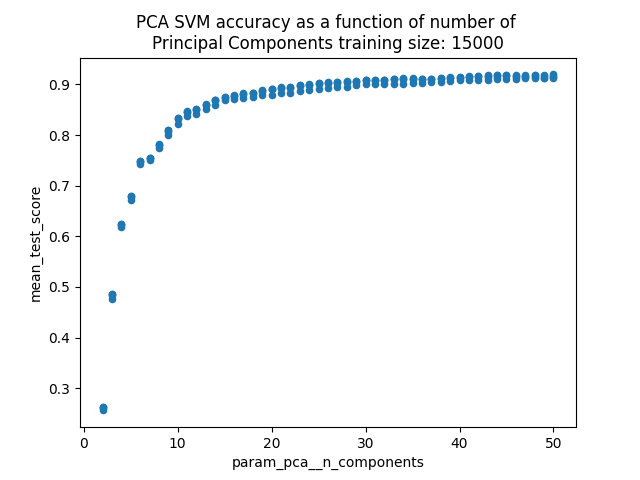
\includegraphics[width=0.8\textwidth]{figures/experiment_two/pca_svm_15000.png}
    \caption{Accuracy of the SVM model with \gls{pca} as dimensionality reduction method, with the number of components used.}
    \label{fig:experiment_2_pca_svm}
\end{figure}

For \gls{pca} the highest accuracy value is 91.9\% with 50 components. Meaning that the thresholds for \gls{pca} are: 91.9\% - 1\% = 90.9, 91.9\% - 5\% = 87.3\%, and 91.9\% - 10\% = 82.7\%. The results of the experiment for \gls{pca} will be compared to these thresholds. 

By sorting the data, by \texttt{mean\_test\_score} and going through the list of values, given the best case scenario for each with the best hyperparamaters found, the first value that drops below the threshold of 90.9\% is with an accuracy of 90.8\% at 31 components. Meaning that the accuracy of the model only increases by 5\% with the last 19 components, which is close to half the total amount of components.
The next threshold of 87.3\% accuracy is found at 87.1\% with 16 components. by removing only 3 components the accuracy dropped from a 1\% loss to a 5\% loss. 
The final threshold of 82.7\% accuracy is found at 82.1\% with 10 components. By removing only 6 components the accuracy dropped from a 5\% loss to a 10\% loss.\todo{Maybe say additional components removed}

\subsubsection{\gls{lda}}\label{subsubsec:experiment_2_lda}
\gls{lda} is another linear dimensionality reduction method, the scatter plot representing this method can be seen in \autoref{fig:experiment_2_lda_svm}. \gls{lda} reduces the dimension to the number of classes $-1$, which is why the total number of components used is 9, since \gls{mnist} has 10 different numbers. The general trend is still valid for discussion in the second experiment.
Simillar to \gls{pca} the accuracy of the model increases as the number of component increases. But arround 6-7 components a noticable drop in accuracy can be seen. The highest accuracy score for \gls{lda} is 87.3\% with 9 components, and the lowest accuracy score is 50.4\% with 2 components. Showing a large difference in accuracy between the best and worst case scenario, with only a few components.

\begin{figure}[htb!]
    \centering
    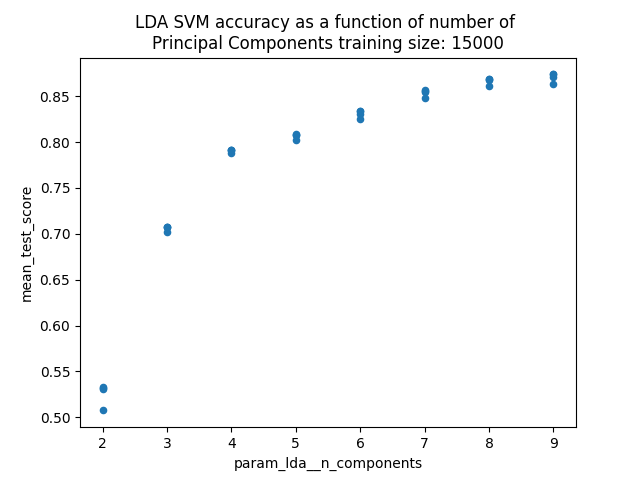
\includegraphics[width=0.8\textwidth]{figures/experiment_two/lda_svm_15000.png}
    \caption{Accuracy of the SVM model with \gls{lda} as dimensionality reduction method, with the number of components used.}
    \label{fig:experiment_2_lda_svm}
\end{figure}

For \gls{lda} the higest accuracy score is at 87.3\% with 9 components. For this the thresholds for \gls{lda} are: 87.3\% - 1\% = 86.3\%, 87.3\% - 5\% = 82.7\%, and 87.3\% - 10\% = 78.1\%. The results of the experiment for \gls{lda} will be compared to these thresholds.

Repeating the method of looking through the data gathered, the first value that drops below the first threshold of 86.3\% is at 86.2\% with 9 components, but with a different hyperparamater set. There are some values with only 8 components that have a higher accuracy score, and some with a lower score than this. Showing the impact of hyperparamater tuning.
The next threshold of 82.7\% accuracy is found at 82.4\% with 6 components. By removing 3 components the accuracy dropped from a 1\% loss to a 5\% loss, which are not many components when compared to \gls{pca}, but for \gls{lda} that only has 9 total components, a third of the components can be removed with a 5\% accuracy loss.
The final threshold of 78.1\% accuracy is found at 70.7\% with only 3 components. Showing a large drop from the threshold, since the first few components have such a large impact on the accuracy score, that the closest value to the threshold is ~8\% away.



\subsubsection{\gls{isomap}}\label{subsubsec:experiment_2_isomap}

\begin{figure}{htb!}
    \centering
    \includegraphics[width=0.8\textwidth]{example-image-a}
    \caption{Accuracy of the SVM model with \gls{isomap} as dimensionality reduction method, with the number of components used.}
    \label{fig:experiment_2_isomap_svm}
\end{figure}


\subsubsection{\gls{kpca}}\label{subsubsec:experiment_2_kpca}

\begin{figure}{htb!}
    \centering
    \includegraphics[width=0.8\textwidth]{example-image-a}
    \caption{Accuracy of the SVM model with \gls{kpca} as dimensionality reduction method, with the number of components used.}
    \label{fig:experiment_2_kpca_svm}
\end{figure}


\subsection{Discussion of experiment two}\label{subsec:experiment_2_discussion}

\subsubsection{Linear methods}

\subsubsection{Non-linear methods}

\subsubsection{Comparison of methods}



% intro
% presentation af de experimenter vi har valgt og hvorfor vi har valgt dem?
% experiment 1 exemple
%     detaljeret gennemgang af regler og evaluering
%     fremvisning af resultater
%     opsumering af resultater
%     diskussion af resultater og hvad der ellers var spændende evaluering af hvorfor det blev sådan.

%logarithmic regression
%Bar chart